% Template of basic phisics experiment 基于 article template，在此基础上做修改
% 设定文章编码类型，正文字号为五号则 zihao=5，正文字号为小四则 zihao=-4
\documentclass[zihao=5, UTF8]{article}		


% 自定义宏定义
\def\N{\mathbb{N}}
\def\F{\mathbb{F}}
\def\Z{\mathbb{Z}}
\def\Q{\mathbb{Q}}
\def\R{\mathbb{R}}
\def\C{\mathbb{C}}
\def\T{\mathbb{T}}
\def\S{\mathbb{S}}
\def\A{\mathbb{A}}
\def\I{\mathscr{I}}
\def\d{\mathrm{d}}
\def\p{\partial}


% 物理实验报告所需的其它宏包
\usepackage{ulem}   % \uline 下划线支持

% 导入基本宏包
\usepackage[UTF8]{ctex}     % 设置文档为中文语言
\usepackage[colorlinks, linkcolor=blue, anchorcolor=blue, citecolor=blue, urlcolor=blue]{hyperref}  % 宏包：自动生成超链接 (此宏包与标题中的数学环境冲突)
% \usepackage{docmute}    % 宏包：子文件导入时自动去除导言区，用于主/子文件的写作方式，\include{./51单片机笔记}即可。注：启用此宏包会导致.tex文件capacity受限。
\usepackage{amsmath}    % 宏包：数学公式
\usepackage{mathrsfs}   % 宏包：提供更多数学符号
\usepackage{amssymb}    % 宏包：提供更多数学符号
\usepackage{pifont}     % 宏包：提供了特殊符号和字体
\usepackage{extarrows}  % 宏包：更多箭头符号

% 列表环境设置
\usepackage{enumitem}   % 宏包：列表环境设置
    \setlist[enumerate]{itemsep=0pt, parsep=0pt, topsep=0pt, partopsep=0pt, leftmargin=3.5em} 
    \setlist[itemize]{itemsep=0pt, parsep=0pt, topsep=0pt, partopsep=0pt, leftmargin=3.5em}
    \newlist{circledenum}{enumerate}{1} % 创建一个新的枚举环境  
    \setlist[circledenum,1]{  
        label=\protect\circled{\arabic*}, % 使用 \arabic* 来获取当前枚举计数器的值，并用 \circled 包装它  
        ref=\arabic*, % 如果需要引用列表项，这将决定引用格式（这里仍然使用数字）
        itemsep=0pt, parsep=0pt, topsep=0pt, partopsep=0pt, leftmargin=3.5em
    }  
% 文章页面 margin 设置
\usepackage[a4paper]{geometry}  % 宏包：文章页面 margin 设置
    \geometry{top=0.75in}
    \geometry{bottom=0.75in}
    \geometry{left=0.75in}
    \geometry{right=0.75in}   % 设置上下左右页边距
    \geometry{marginparwidth=1.75cm}    % 设置边注距离（注释、标记等）

% 自定义数学环境
\usepackage{amsthm} % 宏包：数学环境配置
% theorem-line 环境自定义
    \newtheoremstyle{MyLineTheoremStyle}% <name>
        {11pt}% <space above>
        {11pt}% <space below>
        {}% <body font> 使用默认正文字体
        {}% <indent amount>
        {\bfseries}% <theorem head font> 设置标题项为加粗
        {：}% <punctuation after theorem head>
        {.5em}% <space after theorem head>
        {\textbf{#1}\thmnumber{#2}\ \ (\,\textbf{#3}\,)}% 设置标题内容顺序
    \theoremstyle{MyLineTheoremStyle} % 应用自定义的定理样式
    \newtheorem{LineTheorem}{Theorem.\,}
% theorem-block 环境自定义
    \newtheoremstyle{MyBlockTheoremStyle}% <name>
        {11pt}% <space above>
        {11pt}% <space below>
        {}% <body font> 使用默认正文字体
        {}% <indent amount>
        {\bfseries}% <theorem head font> 设置标题项为加粗
        {：\\ \indent}% <punctuation after theorem head>
        {.5em}% <space after theorem head>
        {\textbf{#1}\thmnumber{#2}\ \ (\,\textbf{#3}\,)}% 设置标题内容顺序
    \theoremstyle{MyBlockTheoremStyle} % 应用自定义的定理样式
    \newtheorem{BlockTheorem}[LineTheorem]{Theorem.\,} % 使用 LineTheorem 的计数器
% definition 环境自定义
    \newtheoremstyle{MySubsubsectionStyle}% <name>
        {11pt}% <space above>
        {11pt}% <space below>
        {}% <body font> 使用默认正文字体
        {}% <indent amount>
        {\bfseries}% <theorem head font> 设置标题项为加粗
        {：\\ \indent}% <punctuation after theorem head>
        {0pt}% <space after theorem head>
        {\textbf{#3}}% 设置标题内容顺序
    \theoremstyle{MySubsubsectionStyle} % 应用自定义的定理样式
    \newtheorem{definition}{}


% 有色文本框及其设置
\usepackage[dvipsnames,svgnames]{xcolor}    %设置插入的文本框颜色
\usepackage[strict]{changepage}     % 提供一个 adjustwidth 环境
\usepackage{framed}     % 实现方框效果
    \definecolor{graybox_color}{rgb}{0.95,0.95,0.96} % 文本框颜色。修改此行中的 rgb 数值即可改变方框纹颜色，具体颜色的rgb数值可以在网站https://colordrop.io/ 中获得。（截止目前的尝试还没有成功过，感觉单位不一样）（找到喜欢的颜色，点击下方的小眼睛，找到rgb值，复制修改即可）
    \newenvironment{graybox}{%
    \def\FrameCommand{%
    \hspace{1pt}%
    {\color{gray}\small \vrule width 2pt}%
    {\color{graybox_color}\vrule width 4pt}%
    \colorbox{graybox_color}%
    }%
    \MakeFramed{\advance\hsize-\width\FrameRestore}%
    \noindent\hspace{-4.55pt}% disable indenting first paragraph
    \begin{adjustwidth}{}{7pt}%
    \vspace{2pt}\vspace{2pt}%
    }
    {%
    \vspace{2pt}\end{adjustwidth}\endMakeFramed%
    }

% 各级标题自定义设置
\usepackage{titlesec}   
    % section标题自定义设置 
    \titleformat{\section}[hang]{\normalfont\huge\bfseries\centering}{第\,\thesection\,部分}{20pt}{}
    % subsection标题自定义设置 
    \titleformat{\subsection}[hang]{\normalfont\Large\bfseries}{\,\thesubsection\,}{8pt}{}
    % subsubsection标题自定义设置
    \titleformat{\subsubsection}[hang]{\normalfont\large\bfseries}{\,\thesubsubsection\,}{6pt}{}

% 外源代码插入设置
\usepackage{matlab-prettifier}
    \lstset{
        style=Matlab-editor,  % 继承matlab代码颜色等
    }
\usepackage[most]{tcolorbox} % 引入tcolorbox包 
\usepackage{listings} % 引入listings包
    \tcbuselibrary{listings, skins, breakable}
    \lstdefinestyle{matlabstyle}{
        language=Matlab,
        basicstyle=\small,
        breakatwhitespace=false,
        breaklines=true,
        captionpos=b,
        keepspaces=true,
        numbers=left,
        numbersep=15pt,
        showspaces=false,
        showstringspaces=false,
        showtabs=false,
        tabsize=2
    }
    \newtcblisting{matlablisting}{
        arc=0pt,
        top=0pt,
        bottom=0pt,
        left=1mm,
        listing only,
        listing style=matlabstyle,
        breakable,
        colback=white   % 选一个合适的颜色
    }

% table 支持
\usepackage{booktabs}   % 宏包：三线表
\usepackage{tabularray} % 宏包：表格排版
\usepackage{longtable}  % 宏包：长表格
\usepackage{tabularx}  % 宏包：宽表格
\usepackage{multirow}  % 宏包：表格中一格显示多个项目

% figure 设置
\usepackage{graphicx}  % 支持 jpg, png, eps, pdf 图片 
\usepackage{svg}       % 支持 svg 图片
    \svgsetup{
        % 指向 inkscape.exe 的路径
        inkscapeexe = C:/aa_MySame/inkscape/bin/inkscape.exe, 
        % 一定程度上修复导入后图片文字溢出几何图形的问题
        inkscapelatex = false                 
    }


% 图表进阶设置
\usepackage{float}     % 图表位置浮动设置 
\usepackage{caption}    % 图注、表注
    \captionsetup[figure]{name=图}  
    \captionsetup[table]{name=表}
    \captionsetup{labelfont=bf, font=small}

% 文章默认字体设置
    \usepackage{fontspec}   % 宏包：字体设置
       \setmainfont{SimSun}    % 设置中文字体为宋体字体
      \setCJKmainfont[AutoFakeBold=3]{SimSun} % 设置加粗字体为 SimSun 族，AutoFakeBold 可以调整字体粗细^     \setmainfont{Times New Roman} % 设置英文字体为Times New Roman


% 其它设置
    % equation 公式编号设置
        \makeatletter  
        \renewcommand{\theequation}{\thesection.\arabic{equation}}  
        \makeatother
    % 脚注设置
        \renewcommand\thefootnote{\ding{\numexpr171+\value{footnote}}}
    % 参考文献引用设置
        \bibliographystyle{unsrt}   % 设置参考文献引用格式为unsrt
        \newcommand{\upcite}[1]{\textsuperscript{\cite{#1}}}     % 自定义上角标式引用
    % 文章序言设置
        \newcommand{\cnabstractname}{序言}
        \newenvironment{cnabstract}{%
            \par\Large
            \noindent\mbox{}\hfill{\bfseries \cnabstractname}\hfill\mbox{}\par
            \vskip 2.5ex
            }{\par\vskip 2.5ex}


% 页眉页脚设置
\usepackage{fancyhdr}   %宏包：页眉页脚设置
    \pagestyle{fancy}
    \fancyhf{}
    \cfoot{\thepage}
    \renewcommand\headrulewidth{1pt}
    \renewcommand\footrulewidth{0pt}
    \rhead{\bfseries 分组序号: YK04-2}    
    \chead{《基础物理实验》实验报告,\ 韩初晓,\ 2023K8009908002}
    \lhead{2024.10.10}

% 文档信息设置
%\title{这里是标题\\The Title of the Report}
%\author{丁毅\\ \footnotesize 中国科学院大学，北京 100049\\ Yi Ding \\ %\footnotesize University of Chinese Academy of Sciences, Beijing %100049, China}
%\date{\footnotesize 2024.8 -- 2025.1}

% 开始编辑文章

\begin{document}
\noindent\begin{flushright}
    \zihao{2}{分组序号: YK04-2}
\end{flushright}

\setCJKfamilyfont{boldsong}[AutoFakeBold = {2.17}]{SimSun}
\newcommand*{\boldsong}{\CJKfamily{boldsong}}


\begin{center}\large
    \noindent{\Huge\bfseries\boldsong《基础物理实验》实验报告 }
    \\\vspace{0.4cm}
    \noindent\textit{
        \textbf{\boldsong 实验名称：}\uline{\hspace{1.7cm} 弦上驻波及介质中声速的测量\hspace{1.7cm}}\hspace{0.4cm} 
        指导教师：\uline{\hspace{1.0cm}吴云\hspace{1.0cm}}}
    \\\vspace{0.1cm}
    \noindent\textit{
        姓名：\uline{\,\,\,韩初晓\,\,\,}\hspace{0.2cm}
        学号：\uline{\,\,\,{\upshape 2023K8009908002}\,\,\,}\hspace{0.2cm}
        专业：\uline{\,\,\,计算机科学与技术\,\,\,}\hspace{0.2cm}
        班级：\uline{\,\,\,\upshape{2306}\,\,\,}}
    \\\vspace{0.1cm}
    \noindent\textit{
        实验日期：\uline{\,\,{\upshape 2024.10.10}\,\,}\hspace{0.2cm}
        实验地点：\uline{\,\,\,教学楼{\upshape713}\,\,\,}\hspace{0.2cm}
        是否调课/补课：\uline{\hspace{0.5cm}否\hspace{0.5cm}}\hspace{0.2cm}
        成绩：\uline{\hspace{2cm}}}
\end{center}
% \vspace{-0.2cm}
\noindent\rule{\textwidth}{0.1em}   % 分割线

% 控制目录不换页
\vspace{1cm}
\setcounter{tocdepth}{2}  % 目录深度为 2（不显示 subsubsection）
\noindent\begin{minipage}{\textwidth}\centering
\tableofcontents\thispagestyle{fancy}   % 显示页码、页眉等   
\end{minipage}  
\newpage

\section{实验目的}

\subsection{弦上驻波实验}

\begin{enumerate}
    \item 探究两端固定的弦线上形成驻波的现象，分析弦线共振以及稳定驻波形成的必要条件。
    
    \item 测量横波在弦线中的传播速度。
    
    \item 通过实验研究弦线在受迫振动下的共振频率如何与半波长的数量 \(n\)、弦的有效长度、张力和线密度相关联。
    
    \item 使用对数坐标绘制共振频率与张力的关系图，采用最小二乘法对实验数据进行线性拟合，并分析结果以得出结论。
\end{enumerate}

\subsection{介质中声速的测量}

\begin{enumerate}
    \item 通过驻波法测量波长。
    
    \item 使用相位差法确定波长。
    
    \item 计算超声波在空气和水中传播的速度。
\end{enumerate}

\section{弦上驻波实验}\thispagestyle{fancy} 

\subsection{实验用具}

\begin{table}[H]
    \centering
    \begin{tabular}{p{3cm} p{10cm}}
        \toprule
        \textbf{仪器/装置} & \textbf{描述} \\
        \midrule
        弦音计 & 
        由以下部分组成：
        \begin{itemize}
            \item 吉他弦、固定吉他弦的支架和基座；
            \item 琴码、砝码支架、砝码；
            \item 驱动线圈和探测线圈。
        \end{itemize}
        驱动线圈通过信号发生器提供的交流信号产生交变磁力，使金属弦线振动；
        探测线圈将弦线的振动转换为电信号，供示波器显示和观察。
        （弦音计的示意图见图 \ref{fig:sonometer}） \\
        \midrule
        信号发生器 & 
        低频功率信号发生器，输出频率范围为 10 Hz 至 1 kHz，
        用于驱动线圈提供一定频率和功率的正弦信号。 \\
        \midrule
        双踪示波器 & 
        用于观察信号源的波形和探测线圈接收到的弦线振动波形，
        便于及时分析弦线的振动现象。 \\
        \bottomrule
    \end{tabular}
    \caption{实验所用仪器与装置}
    \label{tab:equipment_part_1}
\end{table}

\begin{figure}[H]
    \centering
    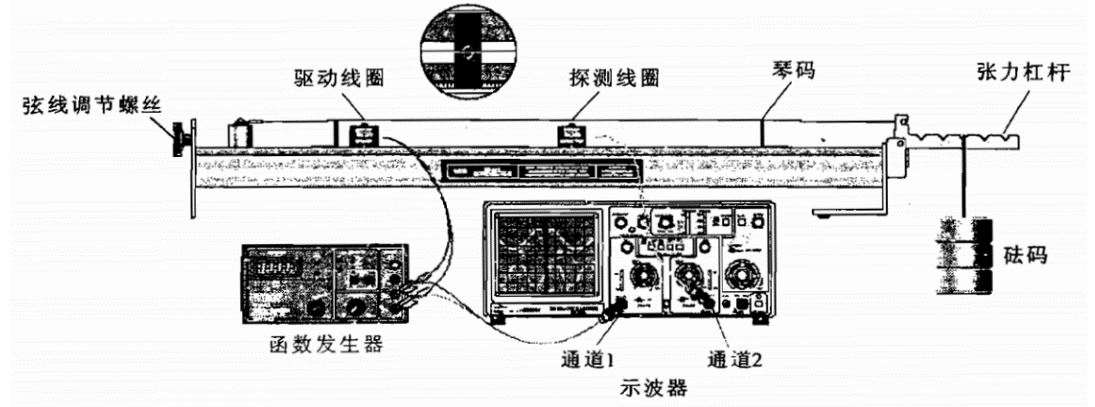
\includegraphics[width=0.6\textwidth]{./弦音计实验总装置图.png}
    \caption{弦音计示意图}
    \label{fig:sonometer}
\end{figure}

\subsection{实验原理}


\subsubsection{驻波的理论基础}

驻波是由两列频率和振幅相等、振动方向相同但传播方向相反的波叠加形成的。设这两列波的波动方程分别为：
\begin{align}
    y_1 &= A \cos(\omega t - kx + \varphi_1) \label{eq:wave1}, \\
    y_2 &= A \cos(\omega t + kx + \varphi_2) \label{eq:wave2},
\end{align}
其中，$k = \frac{2\pi}{\lambda}$ 是波数，$\lambda$ 是波长，$\omega$ 是角频率，$\varphi_1$ 和 $\varphi_2$ 是相位。

两列波叠加后，合成波的表达式为：
\begin{equation}
    y = y_1 + y_2 = 2A \cos\left(\frac{\varphi_2 - \varphi_1}{2} + kx\right) \cos\left(\omega t + \frac{\varphi_1 + \varphi_2}{2}\right). \label{eq:combined_wave}
\end{equation}

从式 \eqref{eq:combined_wave} 可以看出，合成波的振幅由位置 $x$ 决定，其表达式为：
\begin{equation}
    A(x) = 2A \cos\left(\frac{\varphi_1 - \varphi_2}{2} + kx\right). \label{eq:amplitude}
\end{equation}

当 $\cos\left(\frac{\varphi_1 - \varphi_2}{2} + kx\right) = \pm 1$ 时，振幅最大，对应波腹的位置：
\begin{equation}
  x = \pm n\frac{\lambda}{2} \mp \frac{\varphi_2 - \varphi_1}{2k}, \quad n = 0, 1, 2, \ldots \label{eq:antinode}
\end{equation}

当 $\cos\left(\frac{\varphi_1 - \varphi_2}{2} + kx\right) = 0$ 时，振幅为零，对应波节的位置：
\begin{equation}
    x = \pm \left(n + \frac{1}{2}\right)\frac{\lambda}{2} \mp \frac{\varphi_2 - \varphi_1}{2k}, \quad n = 0, 1, 2, \ldots \label{eq:node}
\end{equation}

相邻波腹或波节之间的距离为：
\begin{equation}
    d = \frac{\lambda}{2}.
\end{equation}

\subsubsection{弦上驻波及其特性}

在一根两端固定并施加张力的琴弦上，当机械波沿弦传播并在固定端发生反射时，入射波和反射波叠加，形成驻波。

对于两端固定的弦，驻波的频率满足以下关系：
\begin{equation}
    f_n = n\frac{v}{2L}, \quad n = 1, 2, 3, \ldots \label{eq:resonance_freq}
\end{equation}
其中，$v$ 是波在弦线中的传播速度，$L$ 是弦线的长度，$n$ 是谐波数。$f_1 = \frac{v}{2L}$ 为基频，$f_n$ 为 $n$ 次谐波频率。

根据波动方程，波速 $v$ 与弦的张力 $T$ 和线密度 $\mu$ 的关系为：
\begin{equation}
    v = \sqrt{\frac{T}{\mu}}. \label{eq:wave_speed}
\end{equation}

结合 \eqref{eq:resonance_freq} 和 \eqref{eq:wave_speed}，驻波频率 $f$ 与张力 $T$ 和线密度 $\mu$ 的关系为：
\begin{equation}
    f_n = \frac{n}{2L} \sqrt{\frac{T}{\mu}}. \label{eq:freq_tension_density}
\end{equation}

取对数后可得：
\begin{equation}
    \log f = \frac{1}{2} \log T - \frac{1}{2} \log \mu - \log \lambda. \label{eq:log_relation}
\end{equation}

\subsection{实验内容}

\begin{enumerate}
    \item \textbf{准备琴弦和仪器：}
    \begin{itemize}
        \item 了解弦音计装置的各个组成部分，熟悉每部分的功能与作用。
        \item 在实验前进行必要的调节，确保设备正常工作。熟悉信号发生器和双踪示波器的使用方法。
        \item 通过琴码、张力杠杆、砝码等配件调整琴弦的张力，确保弦线被绷紧并固定长度。调节水平泡，确保张力杆水平，通过力臂测算砝码产生的张力。
    \end{itemize}
    
    \item \textbf{产生入射波并生成驻波：}
    \begin{itemize}
        \item 使用信号发生器通过激振器使琴弦产生振动，逐步调节信号发生器的频率。
        \item 当频率达到合适值时，琴弦上将产生稳定的驻波，能够观察到弦上有明显的振动现象。
    \end{itemize}
    
    \item \textbf{观察并测量驻波的参数：}
    \begin{itemize}
        \item 结合示波器和探测器，测量并记录驻波的频率。
        \item 利用测得的频率计算波速。
        \item 改变频率，探究弦线作受迫振动时的共振频率与半波长个数 $n$ 之间的关系。
    \end{itemize}
    
    \item \textbf{改变琴弦的参数并测量驻波的变化：}
    \begin{itemize}
        \item 改变琴弦的长度 $L$、张力 $T$、线密度 $\mu$ 等参数。
        \item 观察驻波的变化，记录相关数据，并进行分析，验证公式 \eqref{eq:log_relation}。
    \end{itemize}
\end{enumerate}

\subsection{数据整理和计算}

\noindent \textbf{1.线密度测试}\\

首先，测试样品弦的有关性质，数据记录如下表所示：

\begin{table}[H]
	\centering
	\begin{tabular}{|c|c|c|c|c|}
		\hline
		弦号 & 质量（g） & 长度（mm） & 直径（mm） & 线密度（kg/m） \\ \hline
		12 & 0.35 & 61.5 & 1.012 & 0.0057 \\ \hline
	\end{tabular}
	\caption{线密度测试}
  \label{tab:line_density}
\end{table}

\noindent \textbf{2.波速的测量}\\
将琴码放在150mm和650mm的地方，将砝码放在第2\~4格，测基频$f_1$，倍频$f_2$，$f_3$，计算波速的实验值($v=\lambda f $)；根据$v=\sqrt{\frac{T}{\mu}}$计算波速的理论值。通过电子秤的测量，得到砝码质量为506.09g。
\begin{figure}[H]
	\centering
  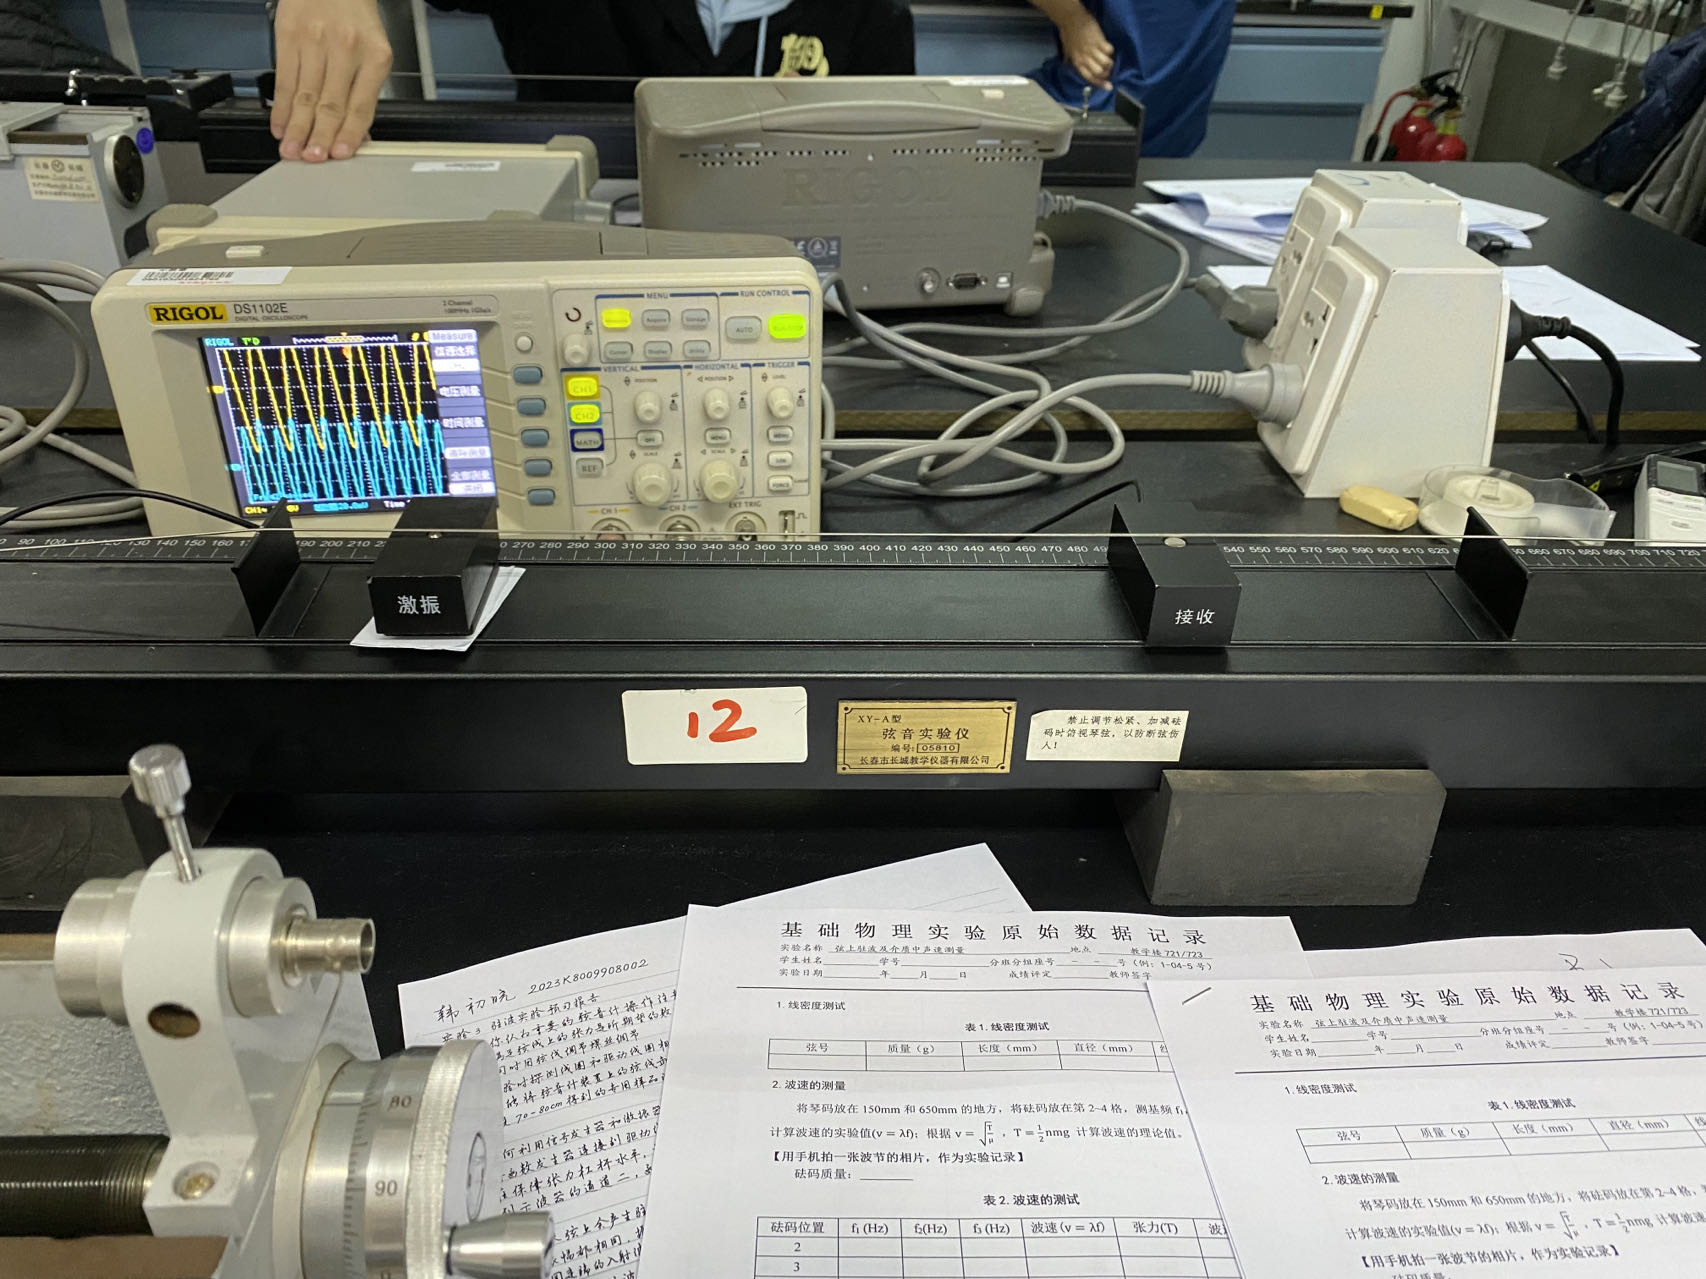
\includegraphics[width=8cm]{./振动的波节.jpg}
	\caption{振动的波节}
\end{figure}

\begin{table}[H]
	\centering
	\begin{tabular}{|>{\centering\arraybackslash}p{1.5cm}|>{\centering\arraybackslash}p{1.5cm}|>{\centering\arraybackslash}p{1.5cm}|>{\centering\arraybackslash}p{1.5cm}|>{\centering\arraybackslash}p{1.5cm}|>{\centering\arraybackslash}p{1.5cm}|>{\centering\arraybackslash}p{1.5cm}|>{\centering\arraybackslash}p{1.5cm}|}
		\hline
		砝码位置 & $f_1$ (Hz) & $f_2$ (Hz) & $f_3$ (Hz) & 波速 ($v = \lambda f$, m/s) & 张力 (T, N) & 实验波速 (m/s) & 相对误差 (\%) \\	
    \hline
    2 & 69.44 & 138.9 & 208.3 & 69.44 & 4.97 & 29.50 & 57.5 \\ \hline
		3 & 86.21 & 172.4 & 263.2 & 86.21 & 7.46 & 36.13 & 58.0 \\ \hline
		4 & 92.59 & 185.3 & 277.8 & 92.59 & 9.94 & 41.72 & 54.9 \\ \hline
	\end{tabular}
	\caption{波速的测量}
  \label{tab:wave_speed}
\end{table}

根据表 \ref{tab:wave_speed} 的数据知道，公式 $\frac{1}{2} nmg$ 已经不再适用。根据测量值波速与实际值波速之间的比较，得到方程
\[
v = \lambda f = \sqrt{\frac{T}{\mu}} = \sqrt{\frac{\alpha nmg}{\mu}}
\]
带入三个测试结果解出参数 $\alpha$ 

\[ \alpha_1 = \frac{v^2 \mu}{nmg} = 2.77\]

\[ \alpha_2 = \frac{v^2 \mu}{nmg} = 2.84\]

\[ \alpha_3 = \frac{v^2 \mu}{nmg} = 2.46\]

取平均值 $\alpha = 2.69$ 。

\noindent
\textbf{3. 频率和有效长度的关系}

\begin{table}[H]
	\centering
	\begin{tabular}{|c|c|c|c|c|c|}
		\hline
		$L$ (mm) & 640 & 480 & 320 & 240 & 160 \\ \hline
		$f_1$ (Hz) & 56.82 & 69.44 & 104.2 & 138.9 & 208.4 \\ \hline
	\end{tabular}
	\caption{频率和有效长度的关系}
\end{table}

根据上述表格，二可以画出频率和有效长度的关系图，如图 \ref{fig:freq_length} 所示。

\begin{figure}[H]
  \centering
  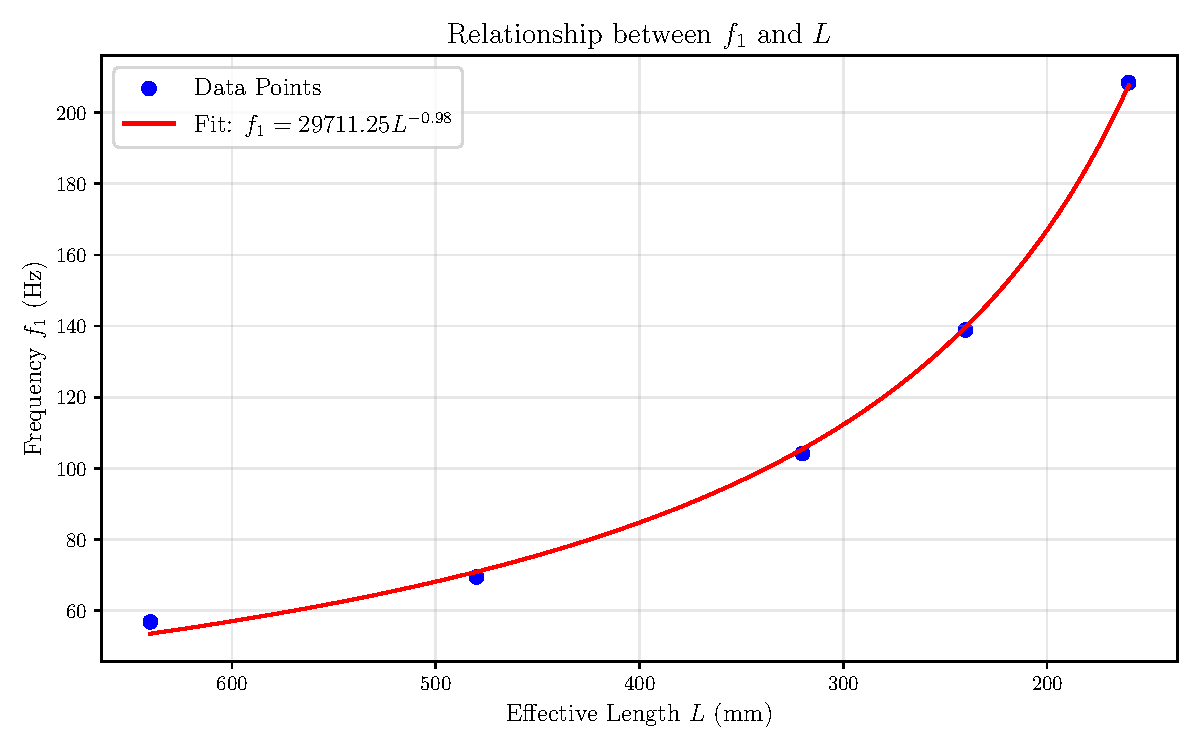
\includegraphics[width=0.6\textwidth]{./频率和有效长度的关系.pdf}
  \caption{频率和有效长度的关系}
  \label{fig:freq_length}
\end{figure}

根据上述曲线可以看出，有效长度越低，频率越高。曲线大致可以用一个负指数函数来拟合。

\noindent \textbf{4. 频率和张力的关系}

固定有效长度为$L=400mm$，将琴码放到$200mm,600mm$的位置，然后将砝码放在 1-5 格时，测量频率 $f_1$ 。得到的图表如下：

\begin{table}[H]
	\centering
	\begin{tabular}{|c|c|c|c|c|c|}
		\hline
		位置 & 1 & 2 & 3 & 4 & 5 \\ \hline
		$T$ (N) & 13.34 & 26.68 & 40.02 & 53.37 & 66.71 \\ \hline
		$f_1$ (Hz) & 65.79 & 83.3 & 98.4 & 111.1 & 135.1 \\ \hline
	\end{tabular}
	\caption{频率和张力的关系}
\end{table}

根据上述表格，可以画出频率和张力的对数之间的关系图，如图 \ref{fig:freq_tension} 所示。

\begin{figure}[H]
  \centering
  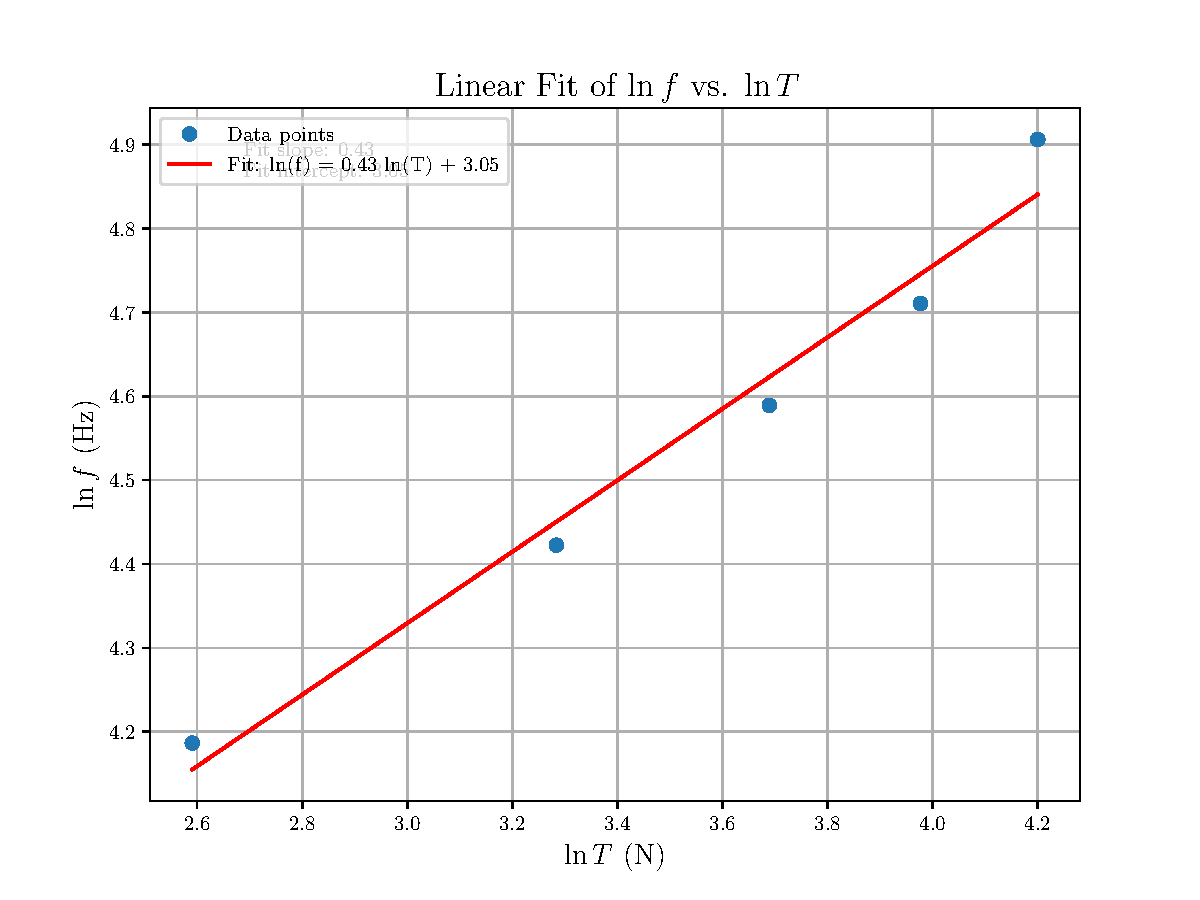
\includegraphics[width=0.6\textwidth]{./频率和张力的关系.pdf}
  \caption{频率和张力的关系}
  \label{fig:freq_tension}
\end{figure}

根据公式 \eqref{eq:log_relation}，可以得到理论上的斜率值为 $0.5$，实验中得到的斜率值为 $0.43$ ，由此计算出相对误差为 $14\%$ 。

\noindent \textbf{5. 频率和线密度的关系}
固定有效长度为$L=400mm$，将琴码放到$200mm,600mm$的位置，同时将砝码固定于第 1 格的位置，测量不同粗细的琴弦的 $f_1$ 。得到的图表如下：

\begin{table}[H]
	\centering
	\begin{tabular}{|c|c|c|c|c|c|}
		\hline
    弦号 & 2 & 3 & 6 & 7 & 11\\ \hline
    直径 (mm) & 0.729 & 1.040 & 0.628 & 0.810 & 0.875 \\ \hline
    $\mu$ (kg/m) & 0.00160 & 0.00558 & 0.00207 & 0.00350 & 0.00375 \\ \hline
		$f_1$ (Hz) & 89.29 & 55.56 & 89.29 & 67.57 & 64.10 \\ \hline
	\end{tabular}
	\caption{频率和线密度之间的关系}
\end{table}

根据上述表格，可以画出频率和线密度的对数之间的关系图，如图 \ref{fig:freq_density} 所示。

\begin{figure}[H]
  \centering
  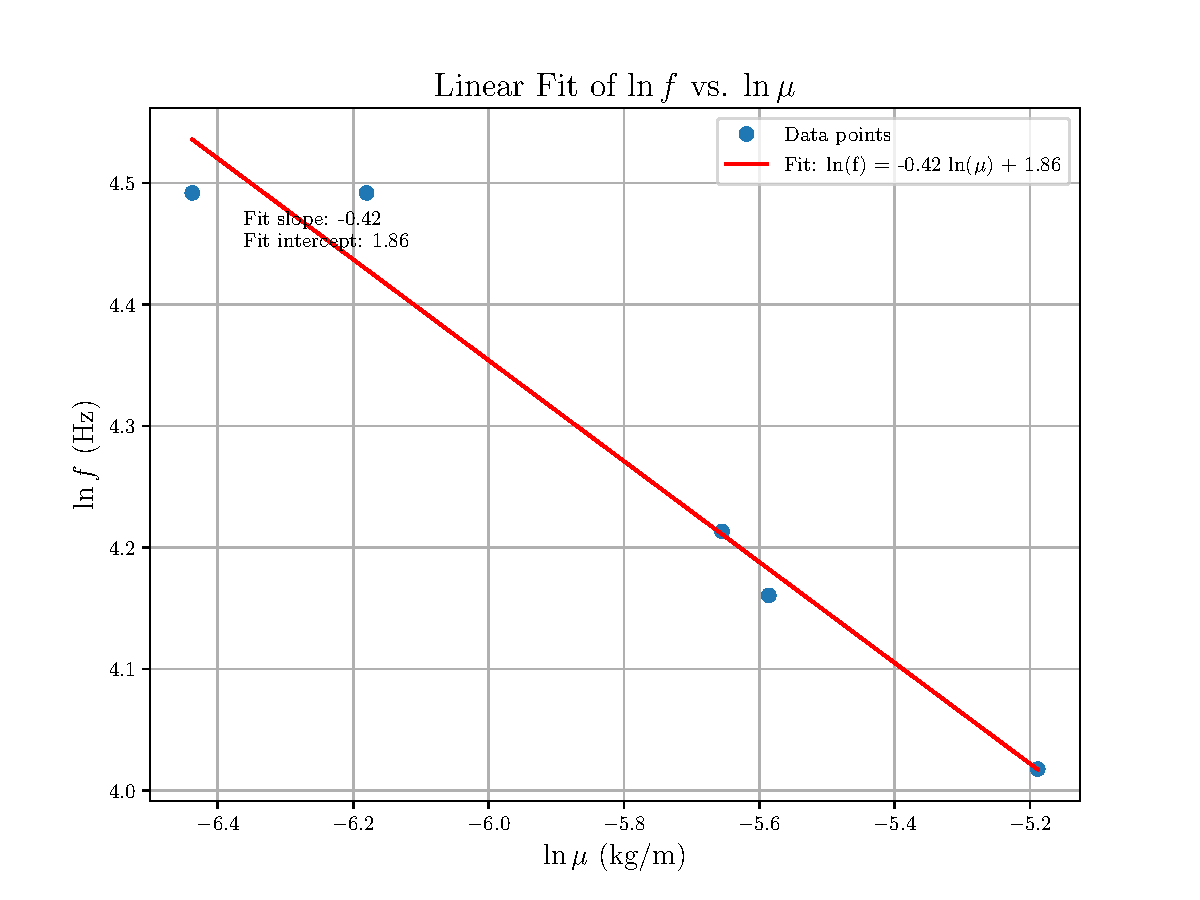
\includegraphics[width=0.6\textwidth]{./频率和线密度的关系.pdf}
  \caption{频率和线密度的关系}
  \label{fig:freq_density}
\end{figure}

根据公式 \eqref{eq:log_relation}，可以得到理论上的斜率值为 $-0.5$，实验中得到的斜率值为 $-0.42$ ，由此计算出相对误差为 $16\%$ 。


\subsection{总结与思考}

\section{介质中声速的测量}

\subsection{实验用具}

\begin{table}[H]
    \centering
    \begin{tabular}{p{3cm} p{10cm}}
        \toprule
        \textbf{仪器/装置} & \textbf{描述} \\
        \midrule
        SW-2 型声速测量仪 & 
        如图 \ref{fig:speed_measurer}所示，声速测量仪包括两个端点：
        \begin{itemize}
            \item 右侧为固定端，安装超声信号发射端；
            \item 左侧为可移动端，安装超声信号接收端，且可以通过鼓轮移动，移动的位置通过标尺读取（读取规则需要参照螺旋测微器的读取规则）。
        \end{itemize}
        调整该装置发射端与接收端之间的距离，示波器上的信号将发生周期性变化 \\
        \midrule
        信号发生器 & 
        用于提供超声信号的频率和功率，驱动声速测量仪中的超声信号发射端。 \\
        \midrule
        示波器 & 
        用于观察由超声信号接收端接收到的信号波形，用于评估鼓轮移动的距离与波长间的关系。 \\
        \bottomrule
    \end{tabular}
    \caption{实验所用仪器与装置}
    \label{tab:equipment_part_2}
\end{table}

\begin{figure}[H]
    \centering
    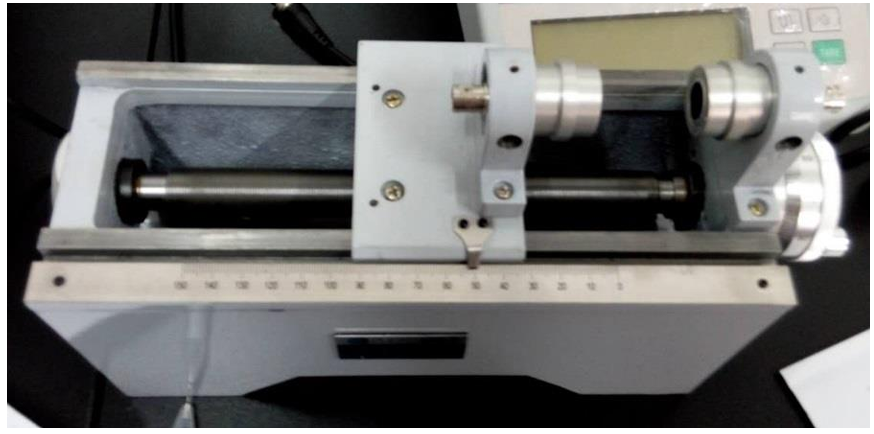
\includegraphics[width=0.6\textwidth]{./声速测量仪.png}
    \caption{SW-2声速测量仪}
    \label{fig:speed_measurer}
\end{figure}

\subsection{实验原理}

\subsubsection{利用驻波法测定声速}

在本实验中，信号发生器输出的正弦电压信号通过电缆传送到超声发射换能器，换能器将电压信号转化为超声波并发射出去。接收换能器则接收声波信号，并将其转化为电压信号，随后输入到示波器进行显示。

根据声波传播的理论，当一定频率的平面声波从发射换能器传播至接收换能器时，如果两者之间的距离等于超声波的整数倍半波长，则会形成驻波。此时，入射波和反射波相互干涉，波腹处声压最小，波节处声压最大。接收换能器的反射界面恰好位于波节位置，声压最大。因此，通过观察接收换能器端面的声压变化，可以判断超声波是否已经形成驻波。

实验中，通过转动鼓轮来改变两换能器之间的距离，在特定的距离点会出现稳定的驻波。每次出现最大电压值时，记录下标尺上的刻度值。相邻两次最大值之间的距离即为半波长 $\frac{\lambda}{2}$。根据公式：
\[
    v = f \lambda,
\]
其中，$f$ 为已知频率，$\lambda$ 为通过实验测得的波长，最终可以计算出超声波在介质中的传播速度 $v$。

\subsubsection{利用相位法测定声速}

在相位法中，实验将发射波和接收波同时输入示波器，并设置为 X-Y 模式显示。两列波的频率相同，但相位不同。当接收器和发射器之间的距离变化等于一个波长时，波的相位差恰好为 $2\pi$。

实验时，通过逐步调整发射器和接收器之间的距离，观察两波之间的相位差变化。每当相位差变化 $\pi$ 时，对应的距离变化即为半波长 $\frac{\lambda}{2}$。利用公式：
\[
    v = f \lambda,
\]
就可以求得声波的传播速度 $v$。

在此过程中，李萨如图形是一个非常重要的工具，能够直观地展示频率相同、相位不同的波形干涉情况（如图  \ref{fig:lisajous} 所示）。

\begin{figure}[H]
    \centering
    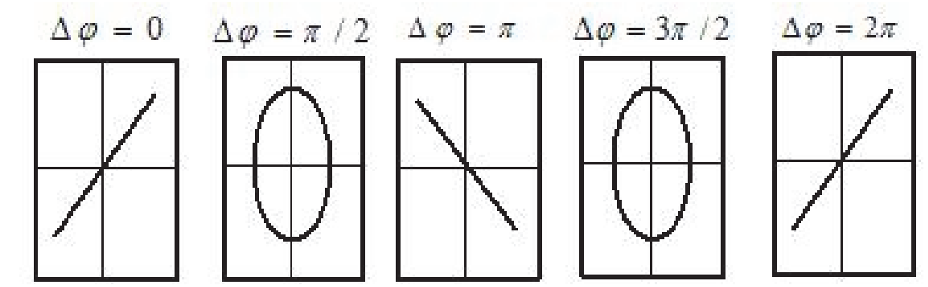
\includegraphics[width=0.6\textwidth]{./李萨如图形.png}
    \caption{李萨如图形}
    \label{fig:lisajous}
\end{figure}

\subsubsection{声速的理论值}

利用声速的理论公式，可以计算空气中声波的理论传播速度。该公式如下：
\[
    v = v_0 \sqrt{\frac{T + 273.15}{T_0 + 273.15}},
\]
其中，$v_0 = 331.45 \, \text{m/s}$ 是 0℃ 时的声速，$T_0 = 0℃$ 是基准温度，$T$ 是当前温度（单位为摄氏度）。


\subsection{实验内容}

\begin{enumerate}
	\item 利用驻波法测超声波在空气中的波速。
	\item 利用相位法测超声波在空气中的波速。
	\item 利用驻波法测超声波在水中的波速。
	\item 利用相位法测超声波在水中的波速。
	\item 利用逐差法处理实验数据。
\end{enumerate}

\subsection{数据整理与计算}

\noindent \textbf{1. 空气中超声波波速的测试}

调节频率为 $f = 40 \, \text{kHz}$，测得室温为 $T = 28.3 \, \text{℃}$ ，根据公式
\[
    v = v_0 \sqrt{\frac{T + 273.15}{T_0 + 273.15}},
\]
知道理论值为 $v = 348.20 \, \text{m/s}$ 。实际实验测得的数据如下表所示：

\begin{table}[H]
	\centering
	\begin{tabular}{|c|c|c|c|c|}
		\hline
		\textbf{} & \textbf{驻波法 $L_i$ (mm)} & \textbf{波长 $\lambda_i$} & \textbf{位相法 $L_i$ (mm)} & \textbf{波长 $\lambda_i$} \\ \hline
		1  & 22.105   & 8.8440  & 20.205  & 9.1364 \\ \hline
		2  & 26.472  & 8.9672 & 25.100  & 8.9596 \\ \hline
		3  & 31.315  & 8.8000  & 29.722  & 8.9132 \\ \hline
		4  & 35.465  & 8.7952 & 34.037  & 8.9816   \\ \hline
		5  & 39.891  & 8.7400  & 38.581  & 8.8740  \\ \hline
		6  & 44.215  & \multirow{5}{*}{8.8293} 
		        & 43.046  & \multirow{5}{*}{8.9729} \\ \cline{1-2} \cline{4-4}
		7  & 48.890  &        & 47.499  &         \\ \cline{1-2} \cline{4-4}
		8  & 53.325  &        & 52.005  &         \\ \cline{1-2} \cline{4-4}
		9  & 57.453  &        & 56.491  &         \\ \cline{1-2} \cline{4-4}
		10 & 61.741  &        & 60.766  &         \\ \hline
		\multicolumn{3}{|c|}{$V = 353.172$ m/s } & \multicolumn{2}{c|}{$V = 358.916$ m/s} \\ \hline
	\end{tabular}
	\caption{驻波法与位相法测量数据}
\end{table}

根据上述数据可知，驻波法测得的声速为 $353.172 \, \text{m/s}$ ，位相法测得的声速为 $358.916 \, \text{m/s}$ 。与理论值 $348.20 \, \text{m/s}$ 相比较，可以计算出相对误差为 $1.43\%$ 和 $3.08\%$ 。

\noindent \textbf{2. 水中超声波波速的测试}

\begin{table}[H]
	\centering
	\begin{tabular}{|c|c|c|}
		\hline
		\textbf{i} & \textbf{刻度值 $L_i$ (mm)} & \textbf{波长 $\lambda$ (mm)} \\ \hline
		1  & 20.427  & 0.8653  \\ \hline
		2  & 20.827  & 0.8984  \\ \hline
		3  & 21.230  & 0.9152  \\ \hline
		4  & 21.657  & 0.9124 \\ \hline
		5  & 22.145  & 0.8904 \\ \hline
		6  & 22.590  & \multirow{5}{*}{0.8963} \\ \cline{1-2}
		7  & 23.073  &        \\ \cline{1-2}
		8  & 23.518  &        \\ \cline{1-2}
		9  & 23.938  &        \\ \cline{1-2}
		10 & 24.371  &        \\ \hline
		\multicolumn{3}{|c|}{\textbf{测量结果：$v = 1523.71$ m/s}} \\ \hline
	\end{tabular}
	\caption{波长测量数据及计算结果}
\end{table}


\subsection{总结与思考}




\end{document}

% VScode 常用快捷键：

% F2:                       变量重命名
% Ctrl + Enter:             行中换行
% Alt + up/down:            上下移行
% 鼠标中键 + 移动:           快速多光标
% Shift + Alt + up/down:    上下复制
% Ctrl + left/right:        左右跳单词
% Ctrl + Backspace/Delete:  左右删单词    
% Shift + Delete:           删除此行
% Ctrl + J:                 打开 VScode 下栏(输出栏)
% Ctrl + B:                 打开 VScode 左栏(目录栏)
% Ctrl + `:                 打开 VScode 终端栏
% Ctrl + 0:                 定位文件
% Ctrl + Tab:               切换已打开的文件(切标签)
% Ctrl + Shift + P:         打开全局命令(设置)

% Latex 常用快捷键：

% Ctrl + Alt + J:           由代码定位到PDF


